\documentclass[12pt]{article}
\usepackage[spanish]{babel}
\usepackage[utf8]{inputenc}
\usepackage{csquotes}

% Interlineado 1.5
\usepackage{setspace}
\onehalfspacing

% Fuente Times New Roman
\usepackage{mathptmx}

% Acomodar margenes del documento
\usepackage[a4paper, margin=2cm, top=3cm, headheight=50pt]{geometry}

% Paquetes comunes
\usepackage{graphicx, float}
\usepackage{amsfonts, amssymb, amsmath}
\usepackage{physics}
\usepackage{enumerate}
\usepackage[colorlinks=true, citecolor=blue]{hyperref}

% Para graficar
\usepackage{pgfplots}
\usepackage{tikz, color}
\usepackage{tikz-3dplot}
\pgfplotsset{width=15cm, compat=1.12}

% Encabezados
\usepackage{fancyhdr}
\pagestyle{fancy}
\fancyhf{}
\fancyfoot[C]{\thepage}
\fancyhead[L]{
  \shortstack[l]{
    {\footnotesize Universidad Tecnológica Nacional} \\
    {\footnotesize Facultad Regional Córdoba} \\
    {\footnotesize Extensión Áulica Bariloche}
  }
}
\fancyhead[C]{
  \shortstack[c]{
    {\footnotesize Fisica 2} \\
    {\footnotesize Resumen Refrigeracion} \\
    {\footnotesize }
  }
}
\fancyhead[R]{
  \shortstack[r]{
    {\footnotesize Profesor: Santiago} \\
    {\footnotesize Alumno: Ricardo Nicolás Freccero} \\
    {\footnotesize Fecha: 26/04/2025}
  }
}

% Para bibliografía
%\usepackage[backend=biber, style=apa]{biblatex}
%\addbibresource{bibliografia.bib}

\begin{document}
\newgeometry{margin=2cm, top=1.5cm}
  \begin{titlepage}
    \centering

    \textsc{
      \LARGE Universidad Tecnológica Nacional\\
      \Large Facultad Regional Córdoba - Extensión Áulica Bariloche\\
      \large Ingeniería en Sistemas de Información\\
      Año lectivo 2025\\[0.5cm]
    }

    \rule{\linewidth}{1.0mm}\\[0.4cm]
    \Huge
    \textbf{Fisica 2}\\
    Resumen Refrigeracion\\[0.2cm]
    \LARGE
    Estoy en clase
    \rule{\linewidth}{1.0mm}\\
    \large
    \begin{flushleft}
      Profesor: Santiago

      Ayudante: Leandro

      Fecha: 26/04/2025
    \end{flushleft}

    \vfill
    \begin{flushright}
      Alumno: Ricardo Nicolás Freccero  

      Número de legajo: 415753
    \end{flushright}
  \end{titlepage}
  
  \restoregeometry
  \tableofcontents
  \newpage

  \section{Segunda Ley de la Termodinamica}
  La priemera ley hablaba de la conservacion de la energia. Un proceso debe cumplir con esta primera ley de la termodinamica. Sin embargo, satisfacer la primera ley no asegura que en realidad el proceso pueda ocurrir.

  Algo que  sabemos que puede pasar es que cuando dejamos una taza de cafe caliente en una habitacion que esta mas fria, esta se enfria tambien hasta llegar a la temperatura de equilibrio. Como la cantidad de energia que pierde el cafe es igual a la que gana la habitacion, esto satisface la primera ley de la termodinamica. Supongamos ahora que pasa al reves; el cafe caliente se vuelve aun mas caliente en una habitacion mas fria como resultado de la transferencia de calor desde el aire. Sabemos que esto nunca pasa, pero en realiadad no viola la primer ley de la termodinamica siempre que lo que se caliente la taza sea lo que se enfria la habitacion.

  Y asi hay un monton de procesos que conocemos, de los cuales podemos concluir que estos procesos van en cierta direccion, pero no es la primera ley la que nos dice eso, sino la segunda ley de la termodinamica.

  \subsection{Maquina termica}
  Convertir el trabajo en calor es sencillo, pero convertiir el calor en trabajo requiere usar algunos dispositivos e speciales. Estos dispositivos se llaman \textbf{maquinas termicas}, y tienen las siguientes caracteristicas:
  \begin{enumerate}[1.]
    \item Reciben calor de una fuente a temperatura alta.

    \item Convierten parte de este calor en trabajo

    \item Rechazan el calor de desecho hacia un sumidero de calor de baja temperatura

    \item Operan en un ciclo
  \end{enumerate}

  Las maquinas termicas y otros dispositivos ciclicos por lo omun reuieren un fluido hacia y desde el cual se transfiere calor mientras experimenta un ciclo. Al fluido se le conoce como \textbf{fluido de trabajo}.

  El dispositivo productor de trabajo que mejor se ajusta a la definicion de maquina termina es la cnetral electrica de vapor.

  Las cantidades mostradas en la figura son:
  \begin{align*}
    Q_{\text{entrada}} &= \text{cantidad de calor suinistrada al vapor en una caldera desde una fuente de temperatura alta (horno).}\\
    Q_{\text{salida}} &= \text{cantidad de calor rechazada del apor en el condesador hacia un sumidero de temperatura baja (atmosfera, rio, etc)}\\
    W_{\text{salida}} &= \text{cantidad de trabajo que entrega el vapor cuando se expande en una turbina}\\
    W_{\text{entrada}} &= \text{cantidad de trabajo requerida para comprimir agua a la presion de la caldera}
  \end{align*}

  \begin{figure}[H]
    \centering
    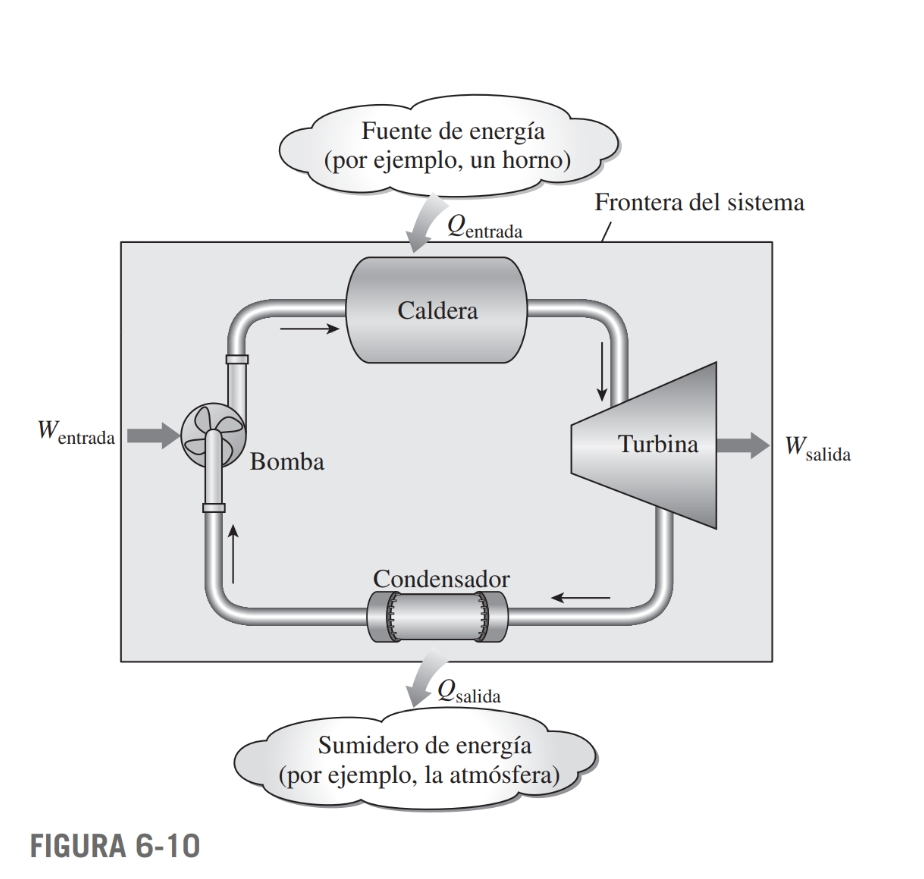
\includegraphics[width=0.5\linewidth]{imagenes/maquina_vapor.jpg}
    \caption{maquina de vapor}
    \label{fig:maq_vapor}
  \end{figure}
  
  La salida del trabajo neto de esta central es la diferencia entre su salida y su entrada.
  \[
  W_{\text{neto, salida}} = W_{\text{salida}} - W_{\text{entrada}}
  \]

  Como nunca entra ni sale masa de este sistema, se puede analizar como un sistema cerrado. Por lo tanto $ \Delta U = 0 $ asi que $ W = Q $. Entonces podemos deducir que:
  \[
  W_{\text{neto, salida}} = Q_{\text{entrada}} - Q_{\text{salida}}
  \]

  \subsection{Eficiencia termica}
  Para las maquinas termicas, la salida deseada es la de trabajo neto, mientras que la entrada que requieren es la cxantidad de calor suministrado al fluido de trabajo. Entonces la eficiencia termina de una maquina termica se puede expresar como:
  \[
  e = \frac{\text{Salida de trabajo neto}}{\text{Entrada de calor total}}
  \]
  entonces tenemos que:
  \[
	  e = \frac{W_{\text{neto,salida}}}{Q_{entrada}}
  \]
  Y ahora podemos reemplazar $ W_{\text{neto, salida}} $:
  \begin{align*}
    e &= \frac{Q_{\text{entradad}} - Q_{\text{salida}}}{Q_{\text{entrada}}}\\
    e &= 1 - \frac{Q_{\text{salida}}}{Q_{\text{entrada}}}
  \end{align*}

  \subsection{Refrigeradores y bombas de calor}
  



  %\addcontentsline{toc}{section}{Referencias}
  %\printbibliography
  
\end{document}
